\documentclass[12pt]{extarticle}
\usepackage[utf8]{inputenc}
\usepackage[main=spanish, english]{babel}
\usepackage{csquotes}
\usepackage{graphicx}
\usepackage{fancyhdr}
\usepackage{geometry}
\usepackage{lipsum}
\usepackage{tocloft} 
\usepackage{amsmath}
\numberwithin{equation}{section}
\setlength{\jot}{14pt}
\usepackage{amssymb}
\usepackage{float}
\usepackage{caption}
\usepackage{pifont}
\usepackage[table,xcdraw]{xcolor}
\usepackage{algpseudocode}
\usepackage{algorithm}
\usepackage{booktabs}
\usepackage{multirow}
\usepackage{listings}
\usepackage{subfiles}

\lstset{
  language=Python,
  basicstyle=\ttfamily\scriptsize,
  keywordstyle=\color{blue},
  stringstyle=\color{teal},
  commentstyle=\color{gray}\itshape,
  numbers=left,
  numberstyle=\tiny,
  frame=none,
  captionpos=b,
  breaklines=true,
  showstringspaces=false
}

\definecolor{darkred}{rgb}{0,0,0}
\definecolor{darkgreen}{rgb}{0,0.8,0}
\definecolor{darkblue}{rgb}{0,0,1}

\usepackage[
    backend=biber,
    style=ieee
]{biblatex}

\addbibresource{ref_tfg.bib}
\addbibresource{ref_executive_summary.bib}

\usepackage{hyperref}
\hypersetup{
    colorlinks,
    linkcolor=darkred,
    filecolor=darkblue,
    urlcolor=darkred,
    citecolor=darkgreen
}

% Language-dependent names
\addto\captionsspanish{
    \renewcommand{\contentsname}{Índice}
    \renewcommand{\listfigurename}{Índice de figuras}
    \renewcommand{\listtablename}{Índice de tablas}
    \renewcommand{\figurename}{Figura}
    \renewcommand{\tablename}{Tabla}
    \renewcommand{\lstlistingname}{Algoritmo}
    \floatname{algorithm}{Algoritmo}
}

\addto\captionsenglish{
    \renewcommand{\contentsname}{Contents}
    \renewcommand{\listfigurename}{List of Figures}
    \renewcommand{\listtablename}{List of Tables}
    \renewcommand{\figurename}{Figure}
    \renewcommand{\tablename}{Table}
    \renewcommand{\lstlistingname}{Algorithm}
    \floatname{algorithm}{Algorithm}
}

% Language-dependent autoref names
\addto\extrasspanish{
    \renewcommand{\tableautorefname}{Tabla}
    \renewcommand{\figureautorefname}{Figura}
    \renewcommand{\equationautorefname}{Ecuación}
    \renewcommand{\sectionautorefname}{Sección}
    \renewcommand{\subsectionautorefname}{Sección}
}

\addto\extrasenglish{
    \renewcommand{\tableautorefname}{Table}
    \renewcommand{\figureautorefname}{Figure}
    \renewcommand{\equationautorefname}{Equation}
    \renewcommand{\sectionautorefname}{Section}
    \renewcommand{\subsectionautorefname}{Section}
}

\newcommand{\blankpage}{
    \clearpage
    \thispagestyle{empty}
    \mbox{}
    \clearpage
}

\usepackage{titlesec}
\usepackage{tocloft}

\titleformat{\section}
  {\normalfont\Large\bfseries}
  {Capítulo \thesection}
  {1em}
  {}

\renewcommand{\cftsecpresnum}{Capítulo~}
\setlength{\cftsecnumwidth}{6em}



%%%%%%%%%%%%%%%%%%%%%%%%%%%%%%%%%%%%%%%%%%%%%%%%%%%%%%%%%%%%%%%%%%%%%%%%%%%%%%%%%%%%%%%%%%%
%%%%%%%%%%%%%%%%%%%%%%%%%%%%%%%%%%%%%%%%%%%%%%%%%%%%%%%%%%%%%%%%%%%%%%%%%%%%%%%%%%%%%%%%%%%
%% CONFIGURATION
%%%%%%%%%%%%%%%%%%%%%%%%%%%%%%%%%%%%%%%%%%%%%%%%%%%%%%%%%%%%%%%%%%%%%%%%%%%%%%%%%%%%%%%%%%%
%%%%%%%%%%%%%%%%%%%%%%%%%%%%%%%%%%%%%%%%%%%%%%%%%%%%%%%%%%%%%%%%%%%%%%%%%%%%%%%%%%%%%%%%%%%

\newcommand{\projectTitle}{T\'itulo del proyecto}
\newcommand{\projectTitleEnglish}{Title of the project}
\newcommand{\Author}{Nombre del estudiante}
\newcommand{\Director}{Nombre del Director}
\newcommand{\CoDirector}{Nombre del co-Director}
\newcommand{\MonthToSubmit}{Mayo }
\newcommand{\BeginYear}{2025}
\newcommand{\EndYear}{\number\numexpr\BeginYear+1\relax }

% Title page command
\newcommand{\ComillasTitlePage}{
\begin{titlepage}
    \centering

    
\includegraphics[width=0.35\textwidth]{images/Logo_comillas.png}\\[1cm] 

    {\Huge \textbf{GRADO EN INGENIER\'IA}}\\[0.3cm]
    {\Huge \textbf{MATEM\'ATICA E INTELIGENCIA}}\\[0.5cm]
    {\Huge \textbf{ARTIFICIAL}}\\[1.5cm]

    {\Huge \textbf{TRABAJO FIN DE GRADO}}\\[1.3cm]

    {\huge \projectTitle}\\[0.5cm]

    \vspace{20mm}

    \textbf{Autor: \Author}\\[1.0cm]
    \textbf{Director: \Director}\\[0.5cm]
    \textbf{Co-Director: \CoDirector}\\

    \raisebox{-2cm}[0cm][0cm]{\large Madrid, \MonthToSubmit \EndYear}

    \vfill
\end{titlepage}
}

\newcommand{\sectionnotoc}[1]{%
    \refstepcounter{section}%
    \section*{\thesection\quad #1}%
}

\newcommand{\resetcounters}{
    \setcounter{section}{0}
    \setcounter{subsection}{0}
    \setcounter{subsubsection}{0}
    \setcounter{figure}{0}
    \setcounter{table}{0}
    \setcounter{equation}{0}
    \setcounter{footnote}{0}
}

\renewcommand{\sectionmark}[1]{%
    \markright{#1}%
}

%%%%%%%%%%%%%%%%%%%%%%%%%%%%%%%%%%%%%%%%%%%%%%%%%%%%%%%%%%%%%%%%%%%%%%%%%%%%%%%%%%%%%%%%%%%
%%%%%%%%%%%%%%%%%%%%%%%%%%%%%%%%%%%%%%%%%%%%%%%%%%%%%%%%%%%%%%%%%%%%%%%%%%%%%%%%%%%%%%%%%%%

\geometry{top=2.5cm, bottom=4cm, left=2.5cm, right=2.5cm}

\begin{document}

\selectlanguage{spanish}

\ComillasTitlePage

\setlength{\headheight}{2cm}

% Configuraci\'on del encabezado
\pagestyle{fancy}
\fancyhf{}

\fancyhead[L]{
\includegraphics[width=2cm]{images/Color_logo_comillas.png}} 

\fancyhead[C]{
    \textbf{UNIVERSIDAD PONTIFICIA COMILLAS}\\
    Escuela T\'ecnica Superior de Ingenier\'ia (ICAI)\\
    Grado en Ingenier\'ia Matem\'atica e Inteligencia Artificial
}

\fancyhead[R]{\small\nouppercase{\rightmark}}

\fancyfoot[C]{\thepage}

\blankpage

\subfile{Anexo_I.tex}

\newpage

\ComillasTitlePage

\blankpage

{\fontsize{17}{20}\selectfont
    \begin{center}
        {\large Agradecimientos}
    \end{center}
    Esta sección es opcional
}

\newpage

%%%%%%%%%%%%%%%%%%%%%%%%%%%%%%%%%%%%%%%%%%%%%%%%%%%%%%%%%%%%%%%%%%%%%%%%%%%%%%%%%%%%%%%%%%%
%% RESUMEN EJECUTIVO IN SPANISH
%%%%%%%%%%%%%%%%%%%%%%%%%%%%%%%%%%%%%%%%%%%%%%%%%%%%%%%%%%%%%%%%%%%%%%%%%%%%%%%%%%%%%%%%%%%

\captionsetup[figure]{list=false}
\captionsetup[table]{list=false}

\begin{otherlanguage}{spanish}

{\large \MakeUppercase{\projectTitle}}
\vspace{3mm}

\textbf{Autor: \Author}

Director: \Director

Co-Director: \CoDirector

\begin{refsection}[ref_executive_summary.bib]

\section*{Resumen}
\textcolor{red}{Este primer párrafo de resumen deberá tener un máximo de 100 palabras unas 7 líneas.}

\textbf{Palabras clave}: \textcolor{red}{Palabra clave 1}; \textcolor{red}{Palabra clave 2}; .... 

\section*{Resumen ejecutivo}
\textcolor{red}{Este apartado completo debe tener una extensi\'on exacta de 3 p\'aginas y sintetizar el problema abordado, el c\'omo se ha resuelto y los resultados m\'as relevantes obtenidos. Se debe incluir al menos una figura de la arquitectura o diseño de la soluci\'on aportada. Este apartado ser\'a uno de los m\'as importantes, ya que podr\'ia ser la \'unica lectura que una persona que desee conocer por encima el alcance del trabajo realice.}

\sectionnotoc{Introducci\'on}

{\color{red}
\begin{itemize}
    \item \textbf{Contexto:} ¿En qué área se sitúa el trabajo? ¿Qué problema general aborda?
    \item \textbf{Motivación:} ¿por qué es importante resolver este problema?
\end{itemize}
}

\sectionnotoc{Objetivos}

{\color{red}
\begin{itemize}
    \item ¿Qué persigue exactamente tu TFG?
    \item ¿Cuál es la pregunta o hipótesis principal?
\end{itemize}
}

\sectionnotoc{Descripci\'on del modelo/sistema/herramienta}

{\color{red}
\begin{itemize}
    \item ¿Cómo has resuelto el problema?
    \item Herramientas, modelos y técnicas empleadas
\end{itemize}

\begin{figure}[h!]
    \centering
    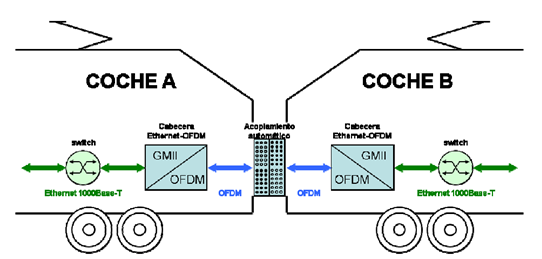
\includegraphics[width=0.5\linewidth]{images/train_schema_example.png}
    \caption{Esquema del sistema conectado de dos vagones contiguos}
    \label{fig:placeholder-es}
\end{figure}

Como se puede ver en la figura \ref{fig:placeholder-es}, ...

}

\sectionnotoc{Resultados}

{\color{red}
\begin{itemize}
    \item ¿C\'omo has validado tu soluci\'on?
    \item ¿Qu\'e resultados has obtenido?
\end{itemize}

\begin{figure}[h!]
    \centering
    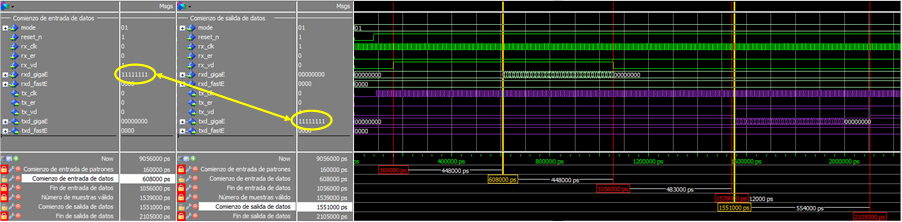
\includegraphics[width=0.5\linewidth]{images/results_example.png}
    \caption{Simulaci\'on del bloque completo de la etapa de frecuencias}
    \label{fig:placeholder2-es}
\end{figure}

Como se puede ver en la figura \ref{fig:placeholder2-es}, ...

}

\sectionnotoc{Conclusiones}

{\color{red}
\begin{itemize}
    \item ¿Qu\'e significan esos resultados?
    \item ¿Cu\'ales son tus principales aportaciones?
\end{itemize}
}

\sectionnotoc{Referencias}

{\color{red}
Incluye las citas necesarias en formato \texttt{bibtex} en el archivo \texttt{ref\_executive\_summary.bib}. Se listar\'an aqu\'i autom\'aticamente seg\'un las utilices usando el comando \texttt{\textbackslash cite} como \cite{einstein1905}.
}

\printbibliography[heading=none]

\end{refsection}

\end{otherlanguage}

\newpage

\resetcounters

%%%%%%%%%%%%%%%%%%%%%%%%%%%%%%%%%%%%%%%%%%%%%%%%%%%%%%%%%%%%%%%%%%%%%%%%%%%%%%%%%%%%%%%%%%%
%% EXECUTIVE SUMMARY IN ENGLISH
%%%%%%%%%%%%%%%%%%%%%%%%%%%%%%%%%%%%%%%%%%%%%%%%%%%%%%%%%%%%%%%%%%%%%%%%%%%%%%%%%%%%%%%%%%%

\begin{otherlanguage}{english}

{\large \MakeUppercase{\projectTitleEnglish}}
\vspace{3mm}

\textbf{Author: \Author}

Director: \Director

Co-Director: \CoDirector

\begin{refsection}[ref_executive_summary.bib]

\section*{Abstract}
\textcolor{red}{This first paragraph of the abstract must have a maximum length of 100 words, approximately 7 lines.}

\textbf{Keywords}: \textcolor{red}{Keyword 1}; \textcolor{red}{Keyword 2}; .... 

\section*{Executive Summary}
\textcolor{red}{This complete section must be exactly 3 pages long and summarize the problem addressed, how it has been solved, and the most relevant results obtained. At least one figure showing the architecture or design of the proposed solution must be included. This section will be one of the most important, since it may be the only section read by someone who wishes to gain a general understanding of the scope of the work.}

\sectionnotoc{Introduction}

{\color{red}
\begin{itemize}
    \item \textbf{Context:} In what area is the work situated? What general problem does it address?
    \item \textbf{Motivation:} Why is it important to solve this problem?
\end{itemize}
}

\sectionnotoc{Objectives}

{\color{red}
\begin{itemize}
    \item What exactly does your Bachelor's Thesis aim to achieve?
    \item What is the main question or hypothesis?
\end{itemize}
}

\sectionnotoc{Description of the Model/System/Tool}

{\color{red}
\begin{itemize}
    \item How have you solved the problem?
    \item Tools, models, and techniques used
\end{itemize}

\begin{figure}[h!]
    \centering
    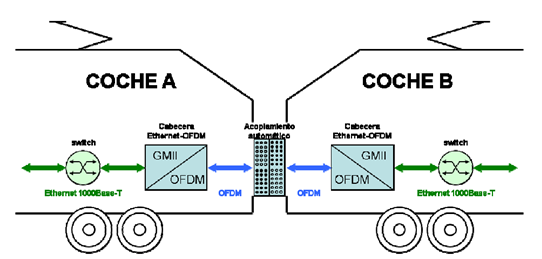
\includegraphics[width=0.5\linewidth]{images/train_schema_example.png}
    \caption{Diagram of the connected system of two adjacent train cars}
    \label{fig:placeholder-en}
\end{figure}

As shown in Figure \ref{fig:placeholder-en}, ...

}

\sectionnotoc{Results}

{\color{red}
\begin{itemize}
    \item How have you validated your solution?
    \item What results have you obtained?
\end{itemize}

\begin{figure}[h!]
    \centering
    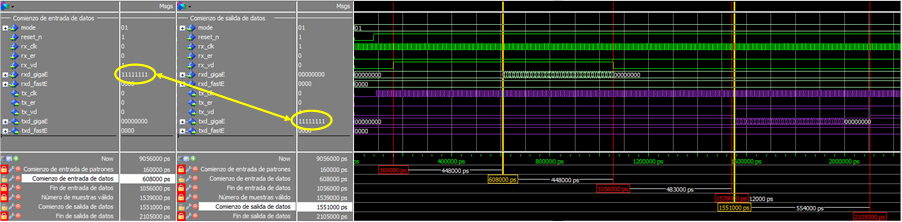
\includegraphics[width=0.5\linewidth]{images/results_example.png}
    \caption{Simulation of the complete block of the frequency stage}
    \label{fig:placeholder2-en}
\end{figure}

As shown in Figure \ref{fig:placeholder2-en}, ...

}

\sectionnotoc{Conclusions}

{\color{red}
\begin{itemize}
    \item What do these results mean?
    \item What are your main contributions?
\end{itemize}
}

\sectionnotoc{References}

{\color{red}
Include the necessary citations in \texttt{bibtex} format in the file \texttt{ref\_executive\_summary.bib}. They will be listed here automatically as you use them with the command \texttt{\textbackslash cite}, as in \cite{einstein1905}.
}

\printbibliography[heading=none]

\end{refsection}

\end{otherlanguage}

\newpage

\captionsetup[figure]{list=true}
\captionsetup[table]{list=true}

\tableofcontents
\thispagestyle{fancy}
\newpage
\setcounter{page}{1}
\fancyfoot[C]{
    \begin{center}
        \thepage
    \end{center}
} 
\renewcommand{\footrulewidth}{0.4pt}
\setlength{\footskip}{0.8cm}

\newpage
\selectlanguage{spanish}

\phantomsection
\listoffigures

\newpage

\phantomsection
\listoftables

\newpage

%%%%%%%%%%%%%%%%%%%%%%%%%%%%%%%%%%%%%%%%%%%%%%%%%%%%%%%%
%%%% Introducci\'on %%%%%%%%%%%%%%%%%%%%%%%%%%%%%%%%%%%%%%
%%%%%%%%%%%%%%%%%%%%%%%%%%%%%%%%%%%%%%%%%%%%%%%%%%%%%%%%

\resetcounters


\begin{refsection}[ref_tfg.bib]
\section{Introducci\'on}
\textcolor{red}{Aqu\'i va la introducci\'on}

\textcolor{blue}{Objetivo de la secci\'on: introducir el problema, por qu\'e debe resolverse este problema y qu\'e mejoras aporta la soluci\'on}



\subsection{Motivaci\'on}
\textcolor{red}{Por qu\'e es importante resolver o resolver parcialmente el vac\'io que has identificado}

\textcolor{blue}{Objetivo de la secci\'on: convencer al lector de que tu proyecto es necesario}

\subsection{Objetivos}
\textcolor{red}{Enumera un objetivo principal y al menos dos objetivos secundarios}

\textcolor{blue}{Objetivo de la secci\'on: definir qu\'e parte exacta del vac\'io resuelves con el proyecto}

\subsection{Alineaci\'on con los ODS}

\textcolor{red}{De los \href{https://sdgs.un.org/es/goals}{Objetivos de Desarrollo Sostenible (ODS)}, enumera aquellos a los que contribuye tu proyecto y justif\'icalo.}

\subsection{Estructura del trabajo}

\textcolor{red}{Explica qu\'e informaci\'on del proyecto se recoge en cada cap\'itulo}

\newpage

%%%%%%%%%%%%%%%%%%%%%%%%%%%%%%%%%%%%%%%%%%%%%%%%%%%%%%%%
%%%% Trabajos relacionados %%%%%%%%%%%%%%%%%%%%%%%%%%%%%
%%%%%%%%%%%%%%%%%%%%%%%%%%%%%%%%%%%%%%%%%%%%%%%%%%%%%%%%
\section{Estado del arte}\label{sec:related} 
{\color{red}
En este capítulo se debe revisar qué trabajos o soluciones existen en el ámbito de mi proyecto. Ante la idea inicial de desarrollar un proyecto, siempre debemos realizarnos la pregunta: ¿hay algo similar en la literatura o en el mercado? ¿Hay algún trabajo de investigación que haya obtenido los resultados que quiero alcanzar?
También hay que indicar cómo se relacionan los trabajos previos con el estudio actual e identificar las áreas que no han sido suficientemente exploradas.
 Este apartado debe dar pie al siguiente, Justificación de mi proyecto. ¿Por qué hago el proyecto?
Por lo tanto, el estado del arte debería cubrir los siguientes aspectos: 

\begin{itemize}
    \item Conceptos fundamentales 
    \item Técnicas y modelos relevantes
    \item Trabajos relacionados (papers, proyectos similares)
    \item Limitaciones de las soluciones actuales.
\end{itemize}
}

\textcolor{blue}{Objetivo de la secci\'on: identificar el vac\'io en el estado del arte en el que vamos a desarrollar la soluci\'on}

\newpage


%%%%%%%%%%%%%%%%%%%%%%%%%%%%%%%%%%%%%%%%%%%%%%%%%%%%%%%%
%%%% Metodolog\'ia %%%%%%%%%%%%%%%%%%%%%%%%%%%%%%%%%%%%%%%
%%%%%%%%%%%%%%%%%%%%%%%%%%%%%%%%%%%%%%%%%%%%%%%%%%%%%%%%
\section{Metodolog\'ia}\label{sec:methodology}

\textcolor{red}{Aqu\'i va la metodolog\'ia / desarrollos / descripci\'on del algoritmo}

\textcolor{blue}{Objetivo de la secci\'on: describir en detalle los desarrollos realizados durante el proyecto, incluyendo desarrollos matem\'aticos y de programaci\'on.}

\subsection{Planteamiento del problema}

\textcolor{red}{
\begin{itemize}
    \item Definición formal del problema
    \item Requisitos
    \item Pruebas y métricas de evaluación para la validación del sistema
\end{itemize}
}

\subsection{Diseño de la soluci\'on}
\textcolor{red}{
\begin{itemize}
    \item Enfoque propuesto 
    \item Arquitectura del sistema 
    \item Algoritmos/modelos utilizados 
    \item Conjuntos de datos utilizados
    \item Justificación técnica 
\end{itemize}
}
\subsection{Implementaci\'on}
\textcolor{red}{
\begin{itemize}
    \item Tecnologías y recursos HW/SW empleados 
    \item Estructura del código 
    \item Pipeline (preprocesado, entrenamiento, evaluación) 
    \item Reproducibilidad
\end{itemize}
}


\newpage

%%%%%%%%%%%%%%%%%%%%%%%%%%%%%%%%%%%%%%%%%%%%%%%%%%%%%%%%
%%%% Experimentos %%%%%%%%%%%%%%%%%%%%%%%%%%%%%%%%%%%%%%%
%%%%%%%%%%%%%%%%%%%%%%%%%%%%%%%%%%%%%%%%%%%%%%%%%%%%%%%%
\section{Resultados}\label{sec:results}

\textcolor{red}{En este capítulo se ha de describir cómo se ha validado la solución y qué resultados se han obtenido según las métricas especificadas en el planteamiento del problema, realizando un análisis crítico de los mismos. También es un capítulo obligatorio y clave, en el que la visualización y la presentación de los resultados serán de suma importancia.
Los resultados obtenidos deberían ser reproducibles, por lo que se deberá aportar toda la información necesaria para ello.
}

\textcolor{blue}{Objetivo de la secci\'on: demostrar cuantitativa y cualitativamente qu\'e tal funcionan los desarrollos realizados}

\newpage

%%%%%%%%%%%%%%%%%%%%%%%%%%%%%%%%%%%%%%%%%%%%%%%%%%%%%%%%
%%%% Conclusiones %%%%%%%%%%%%%%%%%%%%%%%%%%%%%%%%%%%%%%%
%%%%%%%%%%%%%%%%%%%%%%%%%%%%%%%%%%%%%%%%%%%%%%%%%%%%%%%%
\section{Conclusiones y Trabajo Futuro}\label{sec:conclusion}
\textcolor{blue}{Objetivo de la secci\'on: describir en qu\'e medida se han alcanzado los objetivos, en qu\'e otros campos pueden aplicarse los desarrollos, qu\'e mejoras pueden incorporarse al proyecto...}

\newpage

%%%%%%%%%%%%%%%%%%%%%%%%%%%%%%%%%%%%%%%%%%%%%%%%%%%%%%%%
%%%% Referencias %%%%%%%%%%%%%%%%%%%%%%%%%%%%%%%%%%%%%%%
%%%%%%%%%%%%%%%%%%%%%%%%%%%%%%%%%%%%%%%%%%%%%%%%%%%%%%%%
\section{Bibliograf\'ia} \label{sec:bibliography}
\textcolor{red}{Incluye las citas necesarias en formato \texttt{bibtex} en el archivo \texttt{ref\_tfg.bib}. Se listar\'an aqu\'i autom\'aticamente seg\'un las utilices usando el comando \texttt{\textbackslash cite} como \cite{einstein1905}.} 

\printbibliography[heading=none]

\end{refsection}
\newpage

%%%%%%%%%%%%%%%%%%%%%%%%%%%%%%%%%%%%%%%%%%%%%%%%%%%%%%%%
%%%% Anexos %%%%%%%%%%%%%%%%%%%%%%%%%%%%%%%%%%%%%%%%%%%%
%%%%%%%%%%%%%%%%%%%%%%%%%%%%%%%%%%%%%%%%%%%%%%%%%%%%%%%%
\appendix
\section{T\'itulo del Anexo A}
\textcolor{red}{Incluye cuantos anexos sean necesarios. El objetivo de los anexos es incluir informaci\'on importante pero demasiado extensa para incluir en el texto del proyecto (p.ej., gr\'aficas extra o tablas completas de experimentos/hiperpar\'ametros. Pregunta a tu director cuando no est\'es seguro.}

\end{document}




